%%%%%%%%%%%%%%%%%%%%%%%%%%%%%%%%%%%%%%%%%
% Beamer Presentation
% LaTeX Template
% Version 1.0 (10/11/12)
%
% This template has been downloaded from:
% http://www.LaTeXTemplates.com
%
% License:
% CC BY-NC-SA 3.0 (http://creativecommons.org/licenses/by-nc-sa/3.0/)
%
%%%%%%%%%%%%%%%%%%%%%%%%%%%%%%%%%%%%%%%%%

%----------------------------------------------------------------------------------------
%	PACKAGES AND THEMES
%----------------------------------------------------------------------------------------

\documentclass[10pt, aspectratio=169]{beamer} %im 16 zu 9 Format
%\documentclass{beamer} %im 4 zu 3 Format

\mode<presentation> {

% The Beamer class comes with a number of default slide themes
% which change the colors and layouts of slides. Below this is a list
% of all the themes, uncomment each in turn to see what they look like.

%\usetheme{default}
%\usetheme{AnnArbor}
%\usetheme{Antibes}
%\usetheme{Bergen}
%\usetheme{Berkeley}
%\usetheme{Berlin}       %gefällt mir vom Stil gut, ist aber nicht klassisch
%\usetheme{Boadilla}
%\usetheme{CambridgeUS}
%\usetheme{Copenhagen}
%\usetheme{Darmstadt}
%\usetheme{Dresden}
%\usetheme{Frankfurt}
%\usetheme{Goettingen}
%\usetheme{Hannover}
%\usetheme{Ilmenau}
%\usetheme{JuanLesPins}
%\usetheme{Luebeck}
\usetheme{Madrid}     %klassischer Stil, aber nichts besonderes
%\usetheme{Malmoe}
%\usetheme{Marburg}
%\usetheme{Montpellier}
%\usetheme{PaloAlto}
%\usetheme{Pittsburgh}
%\usetheme{Rochester}
%\usetheme{Singapore}
%\usetheme{Szeged}
%\usetheme{Warsaw}

% As well as themes, the Beamer class has a number of color themes
% for any slide theme. Uncomment each of these in turn to see how it
% changes the colors of your current slide theme.

%\usecolortheme{albatross}
%\usecolortheme{beaver}
%\usecolortheme{beetle}
%\usecolortheme{crane}
%\usecolortheme{dolphin}
%\usecolortheme{dove}
%\usecolortheme{fly}
%\usecolortheme{lily}
%\usecolortheme{orchid}
%\usecolortheme{rose}
%\usecolortheme{seagull}
%\usecolortheme{seahorse}
%\usecolortheme{whale}
%\usecolortheme{wolverine}

%\setbeamertemplate{footline} % To remove the footer line in all slides uncomment this line
%\setbeamertemplate{footline}[page number] % To replace the footer line in all slides with a simple slide count uncomment this line

%\setbeamertemplate{navigation symbols}{} % To remove the navigation symbols from the bottom of all slides uncomment this line
}

\usepackage{graphicx} % Allows including images
\usepackage{booktabs} % Allows the use of \toprule, \midrule and \bottomrule in tables
\usepackage{pdfpcnotes}
\usepackage{listings}
\usepackage[ngerman]{datetime}
\usepackage[english, ngerman]{babel}
\usepackage[T1]{fontenc} %Damit Umlaute auch beim Kopieren richtig dargestellt werden
\usepackage{csquotes}

\usepackage{color}

\usepackage{pgfgantt} %GANT Diagramm

% Farbdefinitionen
\definecolor{myblue}{RGB}{0, 51, 102}
\definecolor{myorange}{RGB}{255, 102, 0}

\usepackage{tikz}
\usetikzlibrary{shapes.arrows}

\tikzset{
    myarrow/.style={
        draw,
        fill=orange,
        single arrow,
        minimum height=9ex,
        single arrow head extend=1ex
    }
}

\newcommand{\arrowright}{%
\tikz [baseline=-0.5ex]{\node [myarrow,rotate=0] {};}
}
\newcommand{\arrowleft}{%
\tikz [baseline=-0.5ex]{\node [myarrow,rotate=180] {};}
}

%extra blocks

\newenvironment<>{extrablock}[1]{%
\setbeamercolor{block title}{bg=orange!90!black}%
  \begin{block}#2{#1}}{\end{block}}

\renewcommand{\figurename}{Abbildung}

\lstset{
  basicstyle=\ttfamily,
  columns=fullflexible,
  escapeinside = {(*@}{@*)},
  numbers=left,
  xleftmargin=2.5em,
  frame=single,
  breaklines=true,
}

%Für Zeilenänderungen
\let\origthelstnumber\thelstnumber
\makeatletter
\renewcommand\thelstnumber{%
    \ifnum\value{lstnumber}>0
        \origthelstnumber
    \else
        \ifnum\value{lstnumber}=-1
            \ldots
        \fi
    \fi
}

% for starting line numbers
\newcommand*\startnumber[1]{%
    \setcounter{lstnumber}{\numexpr#1-1\relax}%
}

% for stopping line numbers
\newcommand*\stopnumber{%
    \startnumber{-2}%
}
\makeatother

\usepackage{caption}
\captionsetup{
  figurename=Abb.,
  tablename=Tab.,
  font=scriptsize,
  labelfont=scriptsize
}

%----------------------------------------------------------------------------------------
%	TITLE PAGE
%----------------------------------------------------------------------------------------

\title[Kolloquium]{Entwicklung eines KI-basierten Assistenzsystems mit transparenter Entscheidungsbegründung zur quantitativen Portfoliooptimierung im Wertpapierhandel} % The short title appears at the bottom of every slide, the full title is only on the title page

\author{Jasper Bremenkamp} % Your name
\institute[IU] % Your institution as it will appear on the bottom of every slide, may be shorthand to save space
{
IU Internationale Hochschule \\ % Your institution for the title page
\medskip
\textit{jasper.bremenkamp@iu-study.org}\\ % Your email address
https://jasper.bremenkamp.de
}
\date{31. Oktober 2025} % Date, can be changed to a custom date

\begin{document}

\begin{frame}
    \titlepage % Print the title page as the first slide

    \pnote{=======================================================================================================>}
    \pnote{Hallo und herzlich willkommen zur Präsentation }
    \pnote{meiner Masterarbeit mit dem Titel ...}
    \pnote{Ich, Jasper Bremenkamp, stelle euch das Thema heute}
    \pnote{am  31. Oktober 2025 vor}
\end{frame}

\begin{frame}
  \frametitle{Agenda}
  \tableofcontents

  % Notes hier noch anpassen
  \pnote{0-5}
  \pnote{0.1 Kommen wir zuallerst zur Agenda}
  \pnote{1. Wie üblich starten wir mit der  Einleitung. }
  \pnote{1.1. Hier gehe ich auf Motivation und Zielbild ein, aber grenze schon ab}
  \pnote{2. Dann schauen wir nochmal genauer auf die Problemstellung. }
  \pnote{2.1 Die ich auch bereits in der Einleitung anreiße.}
  \pnote{3. Anschließend erkläre ich kurz das Vorgehen und die eingesetzten Methodiken.}.
  \pnote{4. Darauffolgend die technische Implementierung sowie die Ergebnisse.}
  \pnote{4.1. Dazu gehören das Artefakt bzw Projekt aber auch die Analyse}
  \pnote{5. Und zu guterletzt: Fazit, Reflexion und Ausblick}
\end{frame}

%----------------------------------------------------------------------------------------
%	PRESENTATION SLIDES
%----------------------------------------------------------------------------------------


%--------------------------------
\section{Einleitung}
%--------------------------------
\begin{frame}{Einleitung}
  \begin{columns}
    \column{0.6\textwidth}
    \textbf{Motivation} \\
    \begin{itemize}
      \item Blackbox-Charakter vieler (teil-)automatisierter Systeme im Wertpapierhandel \textrightarrow{} fehlende Nachvollziehbarkeit, geringes Vertrauen.
      \item Anlegerbedürfnis: transparente, begründete Handlungsempfehlungen statt bloßer Signale.
    \end{itemize}
    \vspace{0.1cm}
    \textbf{Zielbild der Arbeit} \\
    \begin{itemize}
      \item KI-Assistenzsystem, das \emph{prozentuale} Empfehlungen zu Einzelwerten mit \emph{natürlichen Begründungen} verknüpft.
      \item Aggregation zu \emph{risikoadaptiver Portfoliosicht} mit Rebalancing-Hinweisen + interaktiver Chat.
    \end{itemize}
    \vspace{0.1cm}
    \textbf{Abgrenzung}
    \begin{itemize}
      \item Entscheidungs\emph{unterstützung}, kein autonomer Trader, Fokus auf Transparenz statt Prognosegenauigkeit.
    \end{itemize}
    \column{0.4\textwidth}
    \begin{figure}
      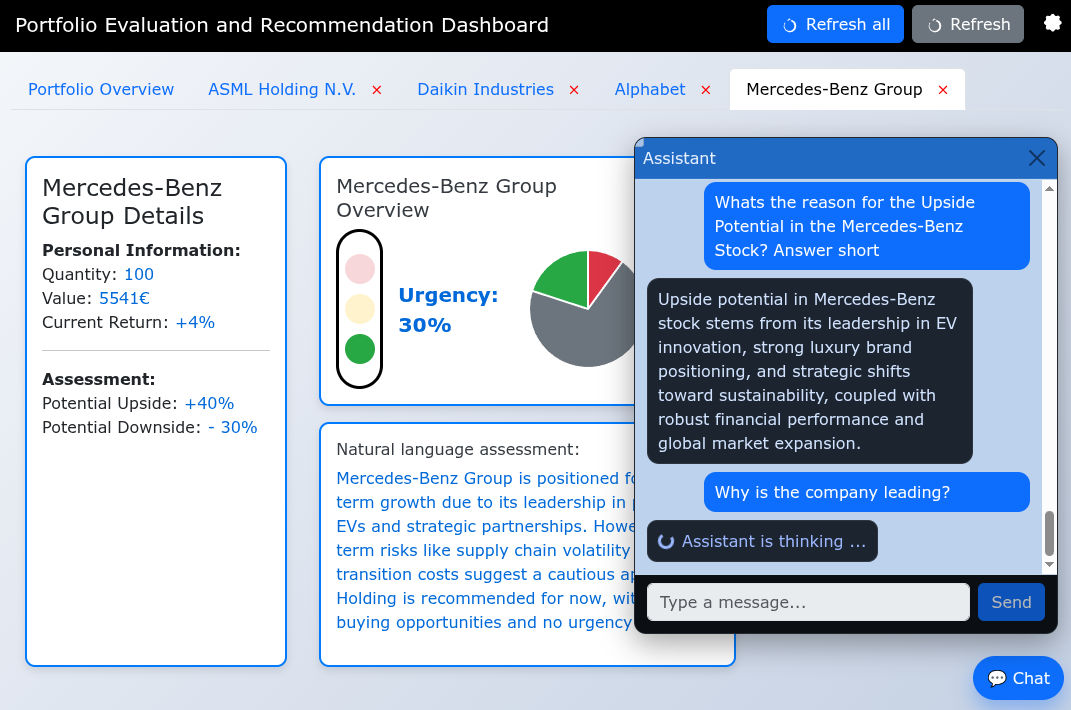
\includegraphics[width=\linewidth]{assets/screenshot_frontend_einzelnes_wertpapier_chat.png}
      \caption{Ausschnitt aus Anwendung (Quelle: Eigene Darstellung)}
    \end{figure}
  \end{columns}

  % Notes am Ende jeder Folie. Nummerieren mit 0 - X (X = letzte Note). Bsp 1-5
  % Das was man Vorlesen kann ohne es von der Folie abzulesen. Nicht 1 zu 1 Inhalts Wiedergabe
  \pnote{=======================================================================================================>}
  \pnote{0-5}
  \pnote{1. Was motiviert die Arbeit?}
  \pnote{1.1 Viele Anleger oder Nutzer im allgemeinen wollen von KI oder oftmals nur Automatisierung }
  \pnote{profitieren. }
  \pnote{1.2 Viele wollen, können und sollten dieser nicht blind vertrauen.}
  \pnote{1.2. Transparenz ist oftmals eine Kernanforderung.}
  \pnote{----}
  \pnote{2. So richtet sich die Forschungsfrage der Arbeit auch nach Transparenz}
  \pnote{ aber auch nach den individuellen Anlagezielen des Nutzers aus }
  \pnote{3. Die Idee: KI liefert quantitative Empfehlungen }
  \pnote{samt verständlichen Begründung im Portfolio-Kontext und erlaubt zudem noch Interaktion.}
  \pnote{----}
  \pnote{4. Der Fokus liegt bewusst auf der unterstützende Rolle.}
  \pnote{4.1. Der Nutzer behält die Verantwortung, keine automatisierte Orderlogik.}
  \pnote{4.2. Es ist ganz bewusst kein Trading-Bot und auch die Prognosegenauigkeit }
  \pnote{der Aussagen steht nur indirekt im Fokus.}
  \pnote{----}
  \pnote{5. Auf den Screenshot gehe ich noch nicht näher ein, dass ist nur ein Vorgeschmack für die späteren Folien }


\end{frame}

%--------------------------------
\section{Problemstellung}
%--------------------------------
\begin{frame}{Problemstellung}
  \begin{enumerate}
    \item \textbf{Erklärungsdefizit in bestehenden Lösungen}
      \begin{itemize}
        \item Prozentempfehlungen ohne kontextspezifische Begründung (z.\,B. Kennzahlen, ESG, Makro-Faktoren).
        \item Wenig Einlfuss auf Aktionen und Anbieterziele vor Nutzerzielen.
      \end{itemize}
    \item \textbf{Portfoliokontext}
      \begin{itemize}
        \item Zu geringe Integration von Einzelanalysen im Gesamtkontext. Gesamtheitlicher Blick fehlt oft.
      \end{itemize}
    \item \textbf{Nutzerzentrierung \& Regulierung}
      \begin{itemize}
        \item Vertrauen, Nachvollziehbarkeit (z.\,B. MiFID-II-Transparenzgedanke).
        \item Unzureichende Nutzerzentrierung und Verantwortung.
      \end{itemize}
  \end{enumerate}
  \vspace{0.2cm}
  \arrowright{} \textbf{Ziel:} Transparentes, modulares System mit begründeten Einzel- \& Portfoliobewertungen als Assistenz.


  % Notes am Ende jeder Folie. Nummerieren mit 0 - X (X = letzte Note). Bsp 1-5
  % Das was man Vorlesen kann ohne es von der Folie abzulesen. Nicht 1 zu 1 Inhalts Wiedergabe
  \pnote{=======================================================================================================>}
  \pnote{0-6}
  \pnote{1. Schauen wir uns die Problemstellung jetzt genauer an.}
  \pnote{2. Da draußen bzw. am Markt gibt es viele Tools.}
  \pnote{2.1 Die allermeisten proprietär. Sprich perse nicht transparent. }
  \pnote{2.2. Entweder bereits in der Bedienung nicht der Öffentlichkeit zugänglich oder falls doch, dann}
  \pnote{dann nur auf eigenen Plattformen mit einer für den Anbieter verbundenen Profitabsicht}
  \pnote{3. Damit mangelt es an Vertrauen und es kann auch nur eingeschränkt nachvollzogen werden}
  \pnote{----}
  \pnote{3.1. Robo-Advisor sind ein hervorragendes Beispiel. Zwar kein Assistent, sondern autonom agierend}
  \pnote{3.2. Begründungen liefert das System zumeist nur kurz und die eigene Verantwortung tritt man ab}
  \pnote{4. Ziel ist es die Verantwortung zu behalten}
  \pnote{2.4. Hier steht Kontrolle im Fokus}
  \pnote{----}
  \pnote{3. Zudem haben viele andere bestehende Tools wie z. B. Aktienscreener nur die Einzelsicht und}
  \pnote{keinen Gesamtkontext.}
  \pnote{4. Um hilfreich zu sein braucht es individuell abgestimmte Empfehlungen, nicht generische }
  \pnote{Markteinschätzungen.}
  \pnote{5. Darüber hinaus gibt es viele Regulatorien wie z. B: MiFID, sodass Nachvollziehbarkeit umso wichtiger wird}
  \pnote{6. KI-Modelle erzeugen plausible Texte -- aber ohne Rahmen oft unstrukturiert und inkonsistent.}
  \pnote{----}
  \pnote{7. Ziel ist ein Transparentes, modulares System, welche Bewertungen begründen kann,}
  \pnote{um effektiv als Assistent zu unterstützen}
  \pnote{8. Das Projekt schafft den Rahmen und der Nutzer bleibt auch weiterhin am Steuer}



\end{frame}

%--------------------------------
\section{Vorgehen und Methodik}
%--------------------------------
\begin{frame}{Vorgehen und Methodik (DSR)}
  \begin{columns}
    \column{0.55\textwidth}
    \textbf{Design Science Research (DSR)}
    \begin{itemize}
      \item Von Problemidentifikation über Konstruktion/Entwicklung zur Evaluation.
      \item Iterative Prototypisierung mit klaren Schnittstellen und Reproduzierbarkeit.
    \end{itemize}
    \vspace{0.2cm}
    \textbf{Technologieauswahl (Nutzwertanalysen)}
    \begin{itemize}
      \item Auswahl \emph{LLM-Anbindung} und \emph{Finanzdaten}-Provider anhand Kriterienkatalogen.
      \item Ziel: Austauschbarkeit, Nachvollziehbarkeit, Betriebspraxis.
    \end{itemize}
    \column{0.45\textwidth}
    \textbf{Evaluationsdesign}
    \begin{itemize}
      \item Konsistenztests der LLM-Ausgaben (Mehrfach-Iterationen).
      \item Abgleich mit Analystenkonsens (Trend/Richtung als Orientierung).
      \item Backtesting: \emph{konzeptionell eingeordnet}, nicht durchgeführt (Scope).
    \end{itemize}
  \end{columns}


  % Notes am Ende jeder Folie. Nummerieren mit 0 - X (X = letzte Note). Bsp 1-5
  % Das was man Vorlesen kann ohne es von der Folie abzulesen. Nicht 1 zu 1 Inhalts Wiedergabe
  \pnote{=======================================================================================================>}
  \pnote{0-10}
  \pnote{0. Nach dem wir die Problemstellung ausreichend beleuchtet haben, kommen wir zum Vorgehen und der Methodik}
  \pnote{----}
  \pnote{1. Vorgegangen wurde nach Design Science Research}
  \pnote{2. Iteratives Vorgehen über Problem zur Konstruktion bishin zur Evaluation}
  \pnote{2. Strukturiertes Vorgehen sichert wissenschaftliche Nachvollziehbarkeit.}
  \pnote{----}
  \pnote{3. Zudem wurde die Nutzwertanalyse bzw Entscheidungsmatrizen eingesetzt.}
  \pnote{3.1. Technologieentscheidungen werden begründet.}
  \pnote{3.2. Keine Auswahl nach Bauchgefühl.}
  \pnote{----}
  \pnote{4. Das Vorgehen in der Evaluation war besonders herausfordernd. }
  \pnote{5. Die Herausforderung lag im Ausmachen der richtigen Evaluationen.}
  \pnote{5.1. Entweder zu umfangreich oder nicht praktikabel realisirbar}
  \pnote{6. Sow wurde auf Konsistenztests und Analystenkonsens zurückgegriffen.}
  \pnote{7. Konsistenztests prüfen Stabilität bei LLM-Ausgaben.}
  \pnote{8. Und der Analystenkonsens dient als Plausibilitätsanker, nicht als Wahrheitsmaß.}
  \pnote{8.1 Denn auch Analysten können falsch liegen. Es geht eher um die allgemeine Tendenz}
  \pnote{9. Erweiterte Verfahren wurden konzeptionell eingeordnet aber nicht durchgeführt}
  \pnote{10. Und nun zur nächsten Folie, der Umsetzung.}

\end{frame}

%--------------------------------
\section{Technische Umsetzung}
%--------------------------------
\begin{frame}{Technische Umsetzung -- Architektur \& Komponenten}
  \begin{columns}

    \column{0.55\textwidth}
    \begin{figure}
        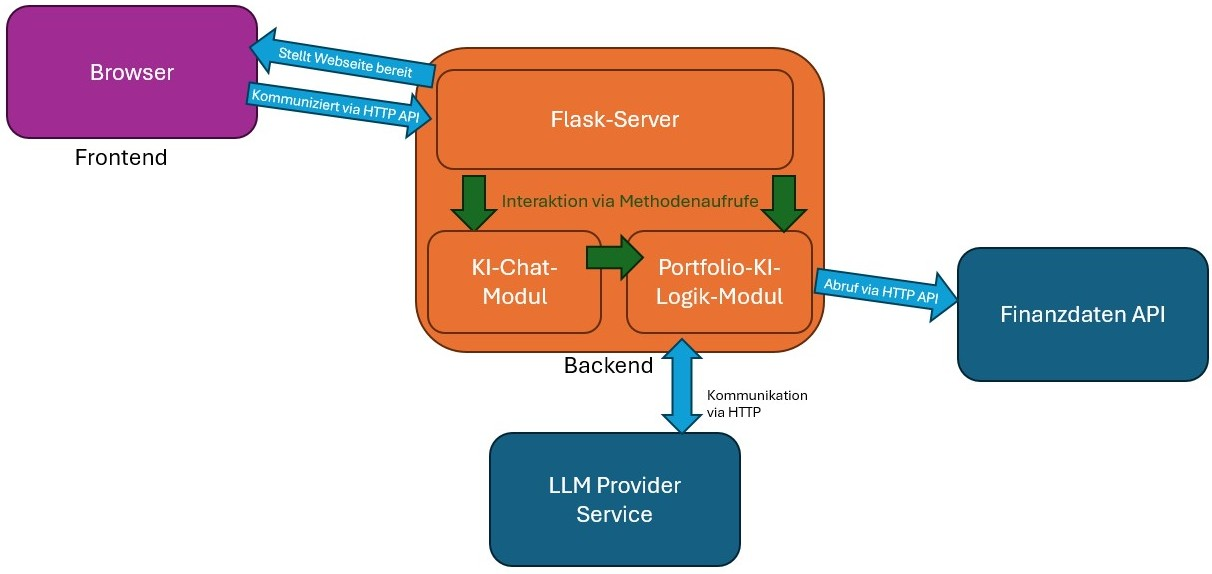
\includegraphics[width=\linewidth]{assets/vereinfachte_systemarchitektur.jpg}
        \caption{Architekturübersicht (Quelle: Eigene Darstellung)}
    \end{figure}

    \column{0.45\textwidth}

    \textbf{Modulare Architektur}
    \begin{itemize}
      \item Backend (Python/Flask) – API \& Logik
      \item LLM-Layer austauschbar (lokal / Cloud)
      \item Finanzdaten und News aus externen APIs
      \item Frontend: Web-UI + Chat
    \end{itemize}

    \vspace{0.2cm}
    \textbf{Qualität \& Entwicklung}
    \begin{itemize}
      \item Prompt-Orchestrierung + Validierung
      \item Fokus: Reproduzierbarkeit \& Transparenz
    \end{itemize}
  \end{columns}

  % Notes am Ende jeder Folie. Nummerieren mit 0 - X (X = letzte Note). Bsp 1-5
  % Das was man Vorlesen kann ohne es von der Folie abzulesen. Nicht 1 zu 1 Inhalts Wiedergabe
  \pnote{0-6}
  \pnote{=======================================================================================================>}
  \pnote{0. Bei der Technische Umsetzung starten wir mit der Architektur.}
  \pnote{1. Architektur trennt Datenbeschaffung, Modelllogik, Ausgabe-Struktur und UI.}
  \pnote{2. LLM-Austauschbarkeit ist gegeben über LangChain (einer Python-Bibliothek),}
  \pnote{die mit den gängigen Providern funktioniert und viele Funktionen mit sich bringt wie z. B. Templates.}
  \pnote{----}
  \pnote{2.1. Das ist wichtig wegen der Schnelllebigkeit der Entwicklung am Markt.}
  \pnote{2.2. Der Code muss nicht direkt an den Anbieter und dessen Änderungen angepasst werden sondern.}
  \pnote{2.2 nur an die Bibliothek, das schafft zudem auch mehr Flexibilät und Kontrolle}
  \pnote{----}
  \pnote{3. Zudem gibt es JSON-Schemas. Erzeugt und validiert mit Pydantic.}
  \pnote{3.1. Diese erzwingen klare Struktur und verhindern LLM-Halluzinationen.}
  \pnote{----}
  \pnote{3.2. Bspw kommt es relativ häufig noch vor, dass das Modell keine 100 Prozent hat.}
  \pnote{4. Die UI ist relativ schlicht, um Fokus auf Entscheidungslogik zu legen.}
  \pnote{5. Ansatz erleichtert Erweiterbarkeit, z.B. durch zusätzliche Module.}
  \pnote{----}
  \pnote{6. Als nächstes gucken wir uns dann den Datenfluss an}


\end{frame}

\begin{frame}{Technische Umsetzung -- Datenfluss}
  \begin{columns}

    \column{0.4\textwidth}

    \begin{block}{Pipeline-Skizze}
      \begin{itemize}
        \item \textbf{Input:} Portfolio, Nutzerziele \& Datenabfrage zur Laufzeit
        \item \textbf{LLM-Orchestrierung:} Strukturierte Prompts mit Validierung (Pydantic)
        \item \textbf{Aggregation:} Gesamtheitliche Portfoliosicht
        \item \textbf{UI \& Interaktivität:} anschließend Visualisierung + Chat für Rückfragen/Erklärungen.
      \end{itemize}
    \end{block}

    \column{0.6\textwidth}

    \vspace*{-0.5cm}

    \begin{figure}
        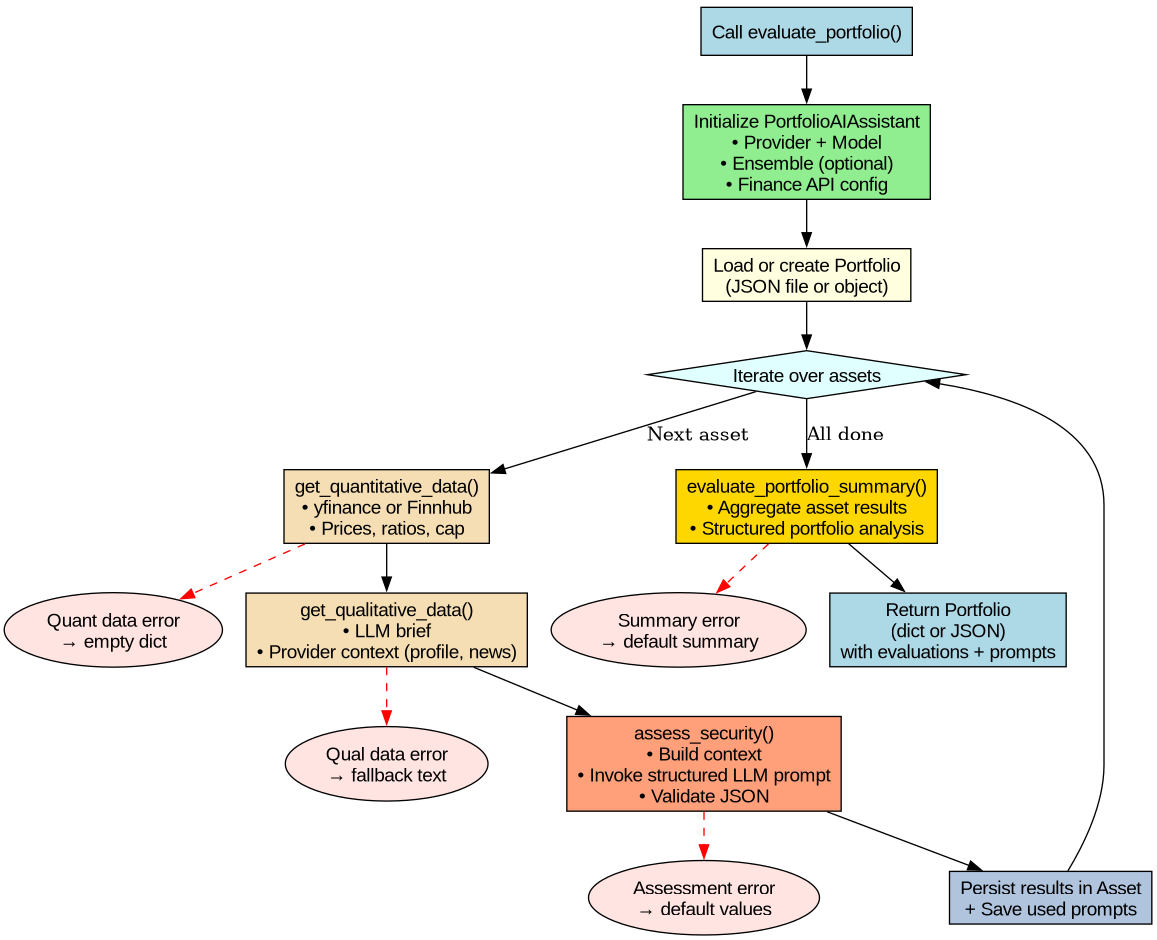
\includegraphics[width=0.9\linewidth]{assets/flowchart_evaluate_portfolio.png}
        \caption{Flow-Chart allgemeiner Ablauf (Quelle: Eigene Darstellung)}
    \end{figure}

  \end{columns}

  % Notes am Ende jeder Folie. Nummerieren mit 0 - X (X = letzte Note). Bsp 1-5
  % Das was man Vorlesen kann ohne es von der Folie abzulesen. Nicht 1 zu 1 Inhalts Wiedergabe
  \pnote{=======================================================================================================>}
  \pnote{0-8}
  \pnote{1. Rechts haben wir einmal einen Flow-Chart der den Ablauf der Hauptkomponente zeigt}
  \pnote{1. Zuallerst werden Objekt und Klasse initialisiert}
  \pnote{2. Anschließend wird das Portfolio geladen.}
  \pnote{----}
  \pnote{3. Jedes Asset bzw. jedes Wertpapier wird dann in einer Schleife vearbeitet}
  \pnote{3.1. Dabei werden quantitative Daten wie Kennzahlen, aber auch quantitative Daten wie News,}
  \pnote{sowie der Portfoliokontext einbezogenund über einen spezielles Prompt-Template bewertet und gespeichert}
  \pnote{----}
  \pnote{4. Und am Ende der Schleife wird das Portfolio gesamtheitlich betrachtet und bewertet.}
  \pnote{5. Kaufen/Verkaufen/Halten sowie die Urgency sind aber nur Durschnittswerte.}
  \pnote{6. Lediglich Erklärungen und Empfehlung werden für das Gesamtportfolio generiert.}
  \pnote{----}
  \pnote{7. Im Anschluss an die Hauptlogik stehen Visualisierung und Chat für Rückfragen und spezifische}
  \pnote{Erklärungen bereit}
  \pnote{8. Und jetzt springen wir zur eigentlichen Anwendung. Ursprünglich hatte ich über eine Live-Demo nachgedacht}
  \pnote{8.1. Aber das Risiko wollte ich meiden. Also bleiben wir bei Screenshots}


\end{frame}

%--------------------------------
\section{Ergebnisse}
%--------------------------------


\begin{frame}{Ergebnisse -- Anwendung (1/3)}

    \begin{figure}
      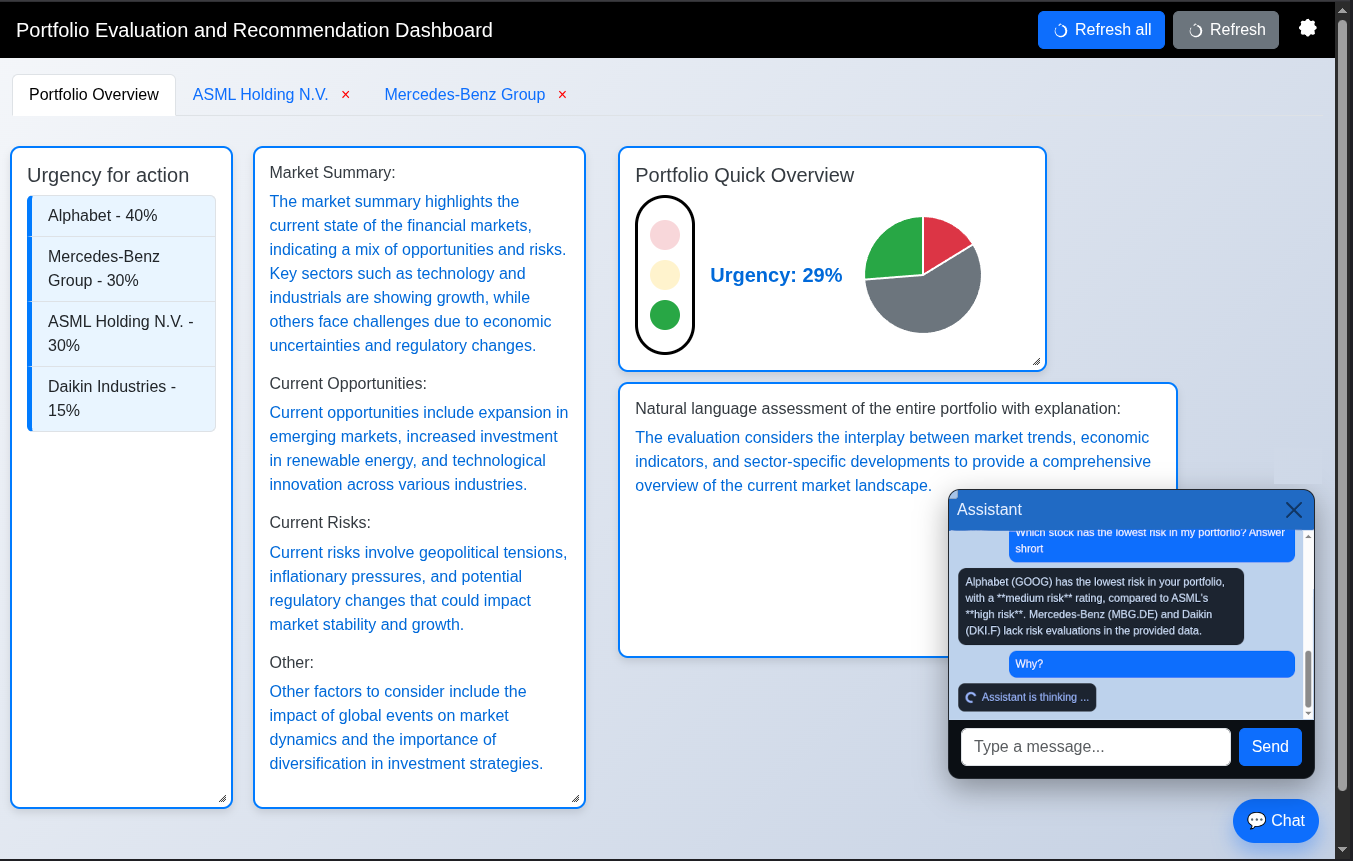
\includegraphics[width=0.7\linewidth]{assets/screenshot_frontend_nach_evaluierung.png}
      \caption{Anwendung -- Übersicht nach Evaluierung (Quelle: Eigene Darstellung)}
    \end{figure}

  % Notes am Ende jeder Folie. Nummerieren mit 0 - X (X = letzte Note). Bsp 1-5
  % Das was man Vorlesen kann ohne es von der Folie abzulesen. Nicht 1 zu 1 Inhalts Wiedergabe
  \pnote{=======================================================================================================>}
  \pnote{0-4}
  \pnote{0. Ich werde jetzt nicht auf jedes einzelne Detail eingehen.}
  \pnote{0.1. Aber es war mir wichtig meine Artefakt auch mal zu zeigen.}
  \pnote{0.2. Da haben wir zuallerst mal die Gesamtübersicht.}
  \pnote{----}
  \pnote{1. Die Oberfläche zeigt das Gesamtportfolio sowie Empfehlungen kompakt.}
  \pnote{1.1 Kaufen/Halten/Verkaufen sind hier nur der Durschnitt der Einzelwerte}
  \pnote{und sind im Tortendiagramm visualisiert}
  \pnote{1.2 Die Dringlichkeit ist ebenfalls gemittelt und wird noch als Ampel angezeigt.}
  \pnote{1.3 Jedes Drittel von 100\% ist eine Farbe}
  \pnote{----}
  \pnote{2. Im Prinzip werden auf der Gesamtübersicht nur generierter Text gezeigt und eben die Zahlen aggregiert}
  \pnote{----}
  \pnote{3. Ziel: Ein guter Überblick über die Gesamtsituation mit der Möglichkeit Wertpapiere anhand ihrer Prio}
  \pnote{auszuwählen}
\end{frame}


\begin{frame}{Ergebnisse -- Anwendung (2/3)}

    \begin{figure}
      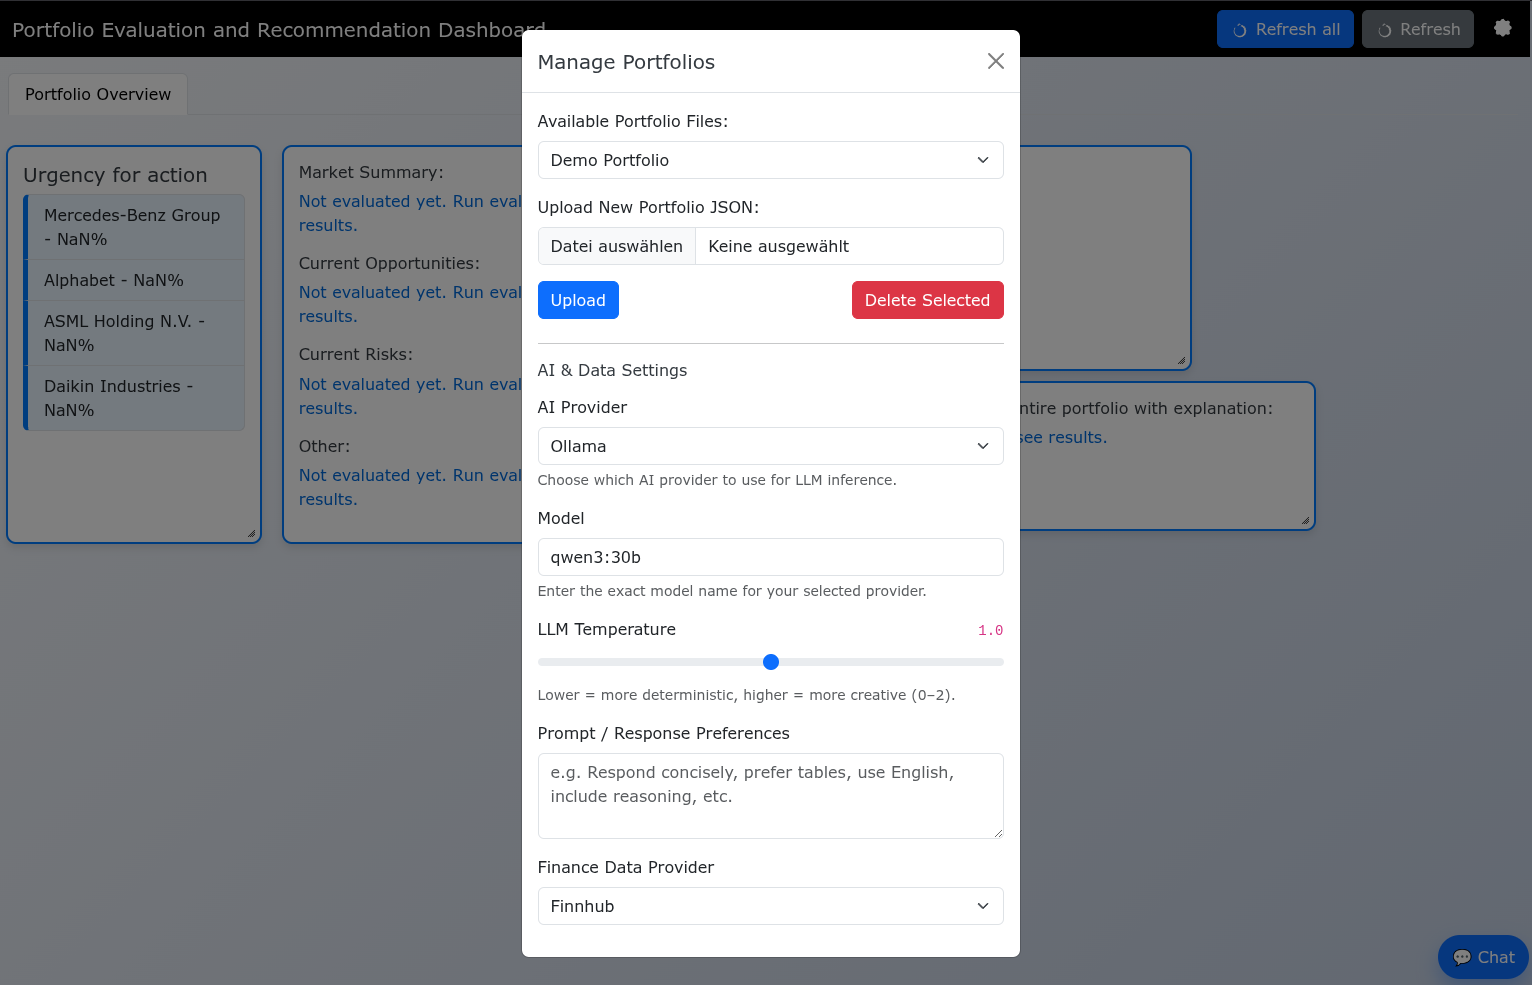
\includegraphics[width=0.7\linewidth]{assets/screenshot_frontend_settings.png}
      \caption{Anwendung -- Einstellungen (Quelle: Eigene Darstellung)}
    \end{figure}

  % Notes am Ende jeder Folie. Nummerieren mit 0 - X (X = letzte Note). Bsp 1-5
  % Das was man Vorlesen kann ohne es von der Folie abzulesen. Nicht 1 zu 1 Inhalts Wiedergabe
  \pnote{0-4}
  \pnote{1. Nutzer definiert Risikoprofil und Anlageziele.}
  \pnote{2. Personalisierung ist wichtig für realen Mehrwert der KI.}
  \pnote{3. Unterschied zu Standard-Finanztools: erklärbare Optimierung statt starrer Profile.}
  \pnote{4. Grundlage für kundenzentrierte KI-Assistenz.}

\end{frame}


\begin{frame}{Ergebnisse -- Anwendung (3/3)}

    \begin{figure}
      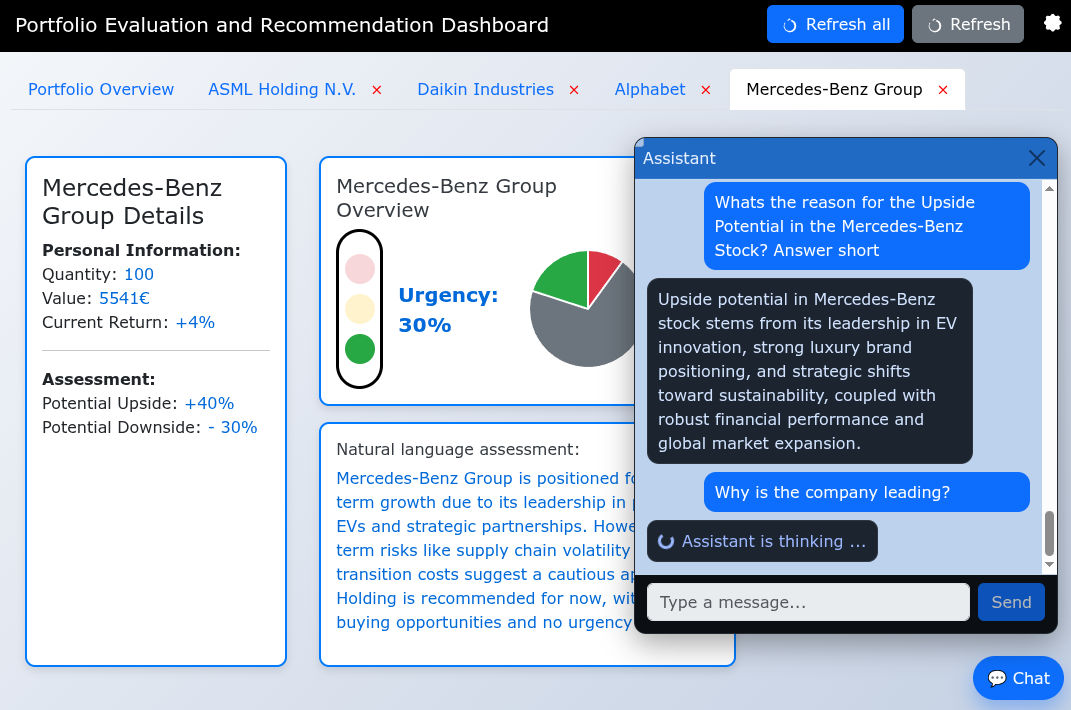
\includegraphics[width=0.68\linewidth]{assets/screenshot_frontend_einzelnes_wertpapier_chat.png}
      \caption{Anwendung -- Einzelansicht  (Quelle: Eigene Darstellung)}
    \end{figure}

  % Notes am Ende jeder Folie. Nummerieren mit 0 - X (X = letzte Note). Bsp 1-5
  % Das was man Vorlesen kann ohne es von der Folie abzulesen. Nicht 1 zu 1 Inhalts Wiedergabe
  \pnote{0-5}
  \pnote{1. Detailanalyse inkl. Prozentvorschlag und Textbegründung.}
  \pnote{2. Chat ermöglicht echte Interaktion statt Einweg-Output.}
  \pnote{3. Nutzer kann Modelle befragen: Erkläre mir das Risiko genauer.}
  \pnote{4. Transparenz in der Argumentation erzeugt Vertrauen.}
  \pnote{5. Werkzeugcharakter statt Automat — Mensch bleibt Entscheider.}


\end{frame}

\begin{frame}{Ergebnisse -- Analyse}
  \begin{alertblock}{Machbarkeit \& Nutzen}
    \begin{itemize}
      \item Kopplung strukturierter Signale mit natürlichsprachlichen Begründungen ist technisch tragfähig.
      \item Portfoliosicht unterstützt \emph{unabhängige Zweitbewertung} vorhandener Einschätzungen.
    \end{itemize}
  \end{alertblock}
  \begin{exampleblock}{Evaluation}
    \begin{itemize}
      \item Konsistenztests: Mehrfachläufe, Vergleich numerischer Ausgaben je Asset/Modell.
      \item Abgleich mit Analystenkonsens: Richtung/Trend als Orientierung, kein Absolutmaß.
    \end{itemize}
  \end{exampleblock}
  \begin{block}{Nicht durchgeführt (Scope)}
    \begin{itemize}
      \item Backtesting nur konzeptionell eingeordnet
      \item Größere Nutzerstudien mit Feedback mangels Kapazität nicht durchführbar
    \end{itemize}
  \end{block}

  % Notes am Ende jeder Folie. Nummerieren mit 0 - X (X = letzte Note). Bsp 1-5
  % Das was man Vorlesen kann ohne es von der Folie abzulesen. Nicht 1 zu 1 Inhalts Wiedergabe
  \pnote{0-6}
  \pnote{1. Konzept technisch umsetzbar und funktionierend.}
  \pnote{2. Konsistenztests zeigen stabile Empfehlungen bei gleichem Kontext.}
  \pnote{3. KI argumentiert plausibel entlang fundamentaler Kennzahlen.}
  \pnote{4. Analystentrends grob getroffen — qualitatives Validationssignal.}
  \pnote{5. Kein Ziel: outperformen, sondern erklären und strukturieren.}
  \pnote{6. Limitationen bewusst gewählt, Fokus auf Nutzbarkeit \& Transparenz.}


\end{frame}

\begin{frame}{Ergebnisse -- Implikationen}
  \begin{block}{Beitrag}
    \begin{itemize}
      \item Konsistentes Vorgehensmodell + modularer Prototyp als belastbare Basis für Erweiterungen/Piloten.
      \item Erhöhte Nachvollziehbarkeit durch klare Schnittstellen, strukturierte Ausgaben, UI-Dialog.
    \end{itemize}
  \end{block}
  \begin{alertblock}{Risiken/Beobachtungen}
    \begin{itemize}
      \item LLM-Stochastik erfordert Konsistenz-Checks \& Parameterdisziplin.
      \item Datenqualität/Aktualität wesentlich für Vertrauen und Reproduzierbarkeit.
    \end{itemize}
  \end{alertblock}

  % Notes am Ende jeder Folie. Nummerieren mit 0 - X (X = letzte Note). Bsp 1-5
  % Das was man Vorlesen kann ohne es von der Folie abzulesen. Nicht 1 zu 1 Inhalts Wiedergabe
  \pnote{0-7}
  \pnote{1. Ziel erreicht: transparente, strukturierte KI-Portfolioassistenz.}
  \pnote{2. Beitrag: nachvollziehbare Investmentargumentation statt Blackbox-ML.}
  \pnote{3. Architektur ist flexibel und marktnah konzipiert.}
  \pnote{4. Limitationen bewusst: keine vollautomatische Trading-Engine.}
  \pnote{5. Zukunft: Backtests, größere Nutzerstudien, Live-News-RAG.}
  \pnote{6. Relevanz steigt mit KI-Regulierung und Anleger-Digitalisierung.}
  \pnote{7. System bereit für Pilotierung im FinTech-/Edu-Kontext.}


\end{frame}

%--------------------------------
\section{Fazit}
%--------------------------------
\begin{frame}{Fazit}
  \begin{itemize}
    \item \textbf{Grundprinzipien}
      \begin{itemize}
        \item Erklärungsorientierte Entscheidungsassistenz statt Blackbox \textrightarrow{} Vertrauen \& Steuerbarkeit.
      \end{itemize}
    \item \textbf{Ergebnisse}
      \begin{itemize}
        \item Funktionsfähiger End-to-End-Prototyp mit Interaktions-UI \& Chat.
        \item Transparenz (begründete Empfehlungen), Austauschbarkeit (Module), Reproduzierbarkeit (JSON/Schemata).
      \end{itemize}
    \item \textbf{Krtische Reflexion}
      \begin{itemize}
        \item Keine großskalige, unabhängige Validierung.
        \item Betriebs-Themen weitestgehend ununtersucht (Latenz/Kosten/Compliance).
      \end{itemize}
    \item \textbf{Aublick}
    \begin{itemize}
      \item Systematische Backtests \& A/B-Studien mit Nutzern.
      \item RAG/Pipeline für aktuelle, qualitativ geprüfte Nachrichten/Research.
      \item Robustheit: Konsistenzmetriken, Prompt-Policies, Model-Governance.
      \item Betrieb: Caching, Kosten-/Latenzoptimierung, Observability, Compliance.
      \end{itemize}
  \end{itemize}

  % Notes am Ende jeder Folie. Nummerieren mit 0 - X (X = letzte Note). Bsp 1-5
  % Das was man Vorlesen kann ohne es von der Folie abzulesen. Nicht 1 zu 1 Inhalts Wiedergabe
  \pnote{0-7}
  \pnote{1. Ziel erreicht: transparente, strukturierte KI-Portfolioassistenz.}
  \pnote{2. Beitrag: nachvollziehbare Investmentargumentation statt Blackbox-ML.}
  \pnote{3. Architektur ist flexibel und marktnah konzipiert.}
  \pnote{4. Limitationen bewusst: keine vollautomatische Trading-Engine.}
  \pnote{5. Zukunft: Backtests, größere Nutzerstudien, Live-News-RAG.}
  \pnote{6. Relevanz steigt mit KI-Regulierung und Anleger-Digitalisierung.}
  \pnote{7. System bereit für Pilotierung im FinTech-/Edu-Kontext.}


\end{frame}

%--------------------------------
\section{Referenzen}
%--------------------------------
\begin{frame}{Referenzen}
  \footnotesize{
  \begin{thebibliography}{99}

        \bibitem[Bremenkamp, 2025]{bremenkamp2025}
        J. Bremenkamp (2025).
        \newblock \emph{Entwicklung eines KI-basierten Assistenzsystems mit transparenter Entscheidungsbegründung
        zur quantitativen Portfoliooptimierung im Wertpapierhandel.}
        Masterarbeit, IU Internationale Hochschule.

  \end{thebibliography}
  }

  % Notes am Ende jeder Folie. Nummerieren mit 0 - X (X = letzte Note). Bsp 1-5
  % Das was man Vorlesen kann ohne es von der Folie abzulesen. Nicht 1 zu 1 Inhalts Wiedergabe
  \pnote{1-1}
  \pnote{1. Sämtliche Inhalte der Folien stammen natürlich aus der Masterarbeit}

\end{frame}

%--------------------------------
\begin{frame}
  \centering \Large Fragen?
  \pnote{Vielen Dank! Ich freue mich auf Ihre Fragen.}
\end{frame}

\end{document}


% To-Dos:
  % 15min gut erreichbar
  % Notizen noch vervollständigen und Potentielle Fragen bereits ausdenken und vorbereiten